%%%%%%%%%%%%%%%%%%%%%%%%%%%%%%%%%%%%%%%%%
% University/School Laboratory Report
% LaTeX Template
% Version 3.1 (25/3/14)
%
% This template has been downloaded from:
% http://www.LaTeXTemplates.com
%
% Original author:
% Linux and Unix Users Group at Virginia Tech Wiki 
% (https://vtluug.org/wiki/Example_LaTeX_chem_lab_report)
%
% License:
% CC BY-NC-SA 3.0 (http://creativecommons.org/licenses/by-nc-sa/3.0/)
%
%%%%%%%%%%%%%%%%%%%%%%%%%%%%%%%%%%%%%%%%%

%----------------------------------------------------------------------------------------
%	PACKAGES AND DOCUMENT CONFIGURATIONS
%----------------------------------------------------------------------------------------

\documentclass{article}

\usepackage[version=3]{mhchem} % Package for chemical equation typesetting
\usepackage{siunitx} % Provides the \SI{}{} and \si{} command for typesetting SI units
\usepackage{graphicx} % Required for the inclusion of images
\usepackage{natbib} % Required to change bibliography style to APA
\usepackage{amsmath} % Required for some math elements 
\usepackage[table,xcdraw]{xcolor}
\usepackage{listings}
\usepackage{hyperref}
\usepackage{xcolor}
\usepackage{color} %red, green, blue, yellow, cyan, magenta, black, white
\definecolor{mygreen}{RGB}{28,172,0} % color values Red, Green, Blue
\definecolor{mylilas}{RGB}{170,55,241}
\lstset{language=Matlab,%
    %basicstyle=\color{red},
    breaklines=true,%
    morekeywords={matlab2tikz},
     backgroundcolor=\color{black!5}, % set backgroundcolor
    keywordstyle=\color{blue},%
    morekeywords=[2]{1}, keywordstyle=[2]{\color{black}},
    identifierstyle=\color{black},%
    stringstyle=\color{mylilas},
    commentstyle=\color{mygreen},%
    showstringspaces=false,%without this there will be a symbol in the places where there is a space
    numbers=left,%
    numberstyle={\tiny \color{black}},% size of the numbers
    numbersep=9pt, % this defines how far the numbers are from the text
    emph=[1]{for,end,break},emphstyle=[1]\color{red}, %some words to emphasise
    %emph=[2]{word1,word2}, emphstyle=[2]{style},    
}

\usepackage[utf8]{inputenc} %Türkçe karakterler
\usepackage{floatrow}
\usepackage{geometry}
\usepackage{caption}
\usepackage{subcaption}
\geometry{margin=1in}

\renewcommand{\lstlistingname}{Code Snippet}

%\setlength\parindent{0pt} % Removes all indentation from paragraphs

% Table float box with bottom caption, box width adjusted to content
\newfloatcommand{capbtabbox}{table}[][\FBwidth]


%\usepackage{times} % Uncomment to use the Times New Roman font

%----------------------------------------------------------------------------------------
%	DOCUMENT INFORMATION
%----------------------------------------------------------------------------------------

\title{Assignment 2: \\ Panorama Stitching\\ COMP 408} % Title

\author{Ahmet \textsc{Uysal}} % Author name

\date{\today} % Date for the report

\begin{document}

\maketitle % Insert the title, author and date

\begin{center}
\begin{tabular}{l r}
Instructor: & Y\"ucel  \textsc{Yemez} % Instructor/supervisor
\end{tabular}
\end{center}

% If you wish to include an abstract, uncomment the lines below
% \begin{abstract}
% Abstract text
% \end{abstract}


\section{Feature Detection}	
\subsection{Algorithm}
The code for this part was given in the assignment. Basically, differences of Gaussian filters are applied to image in different scales to detect set of key points, each associated with a best scale. Later, these key points will be used for creating SIFT descriptors.

\subsection{Sample Outputs}
\begin{figure}[!htb]
\begin{subfigure}{.5\textwidth}
  \centering
  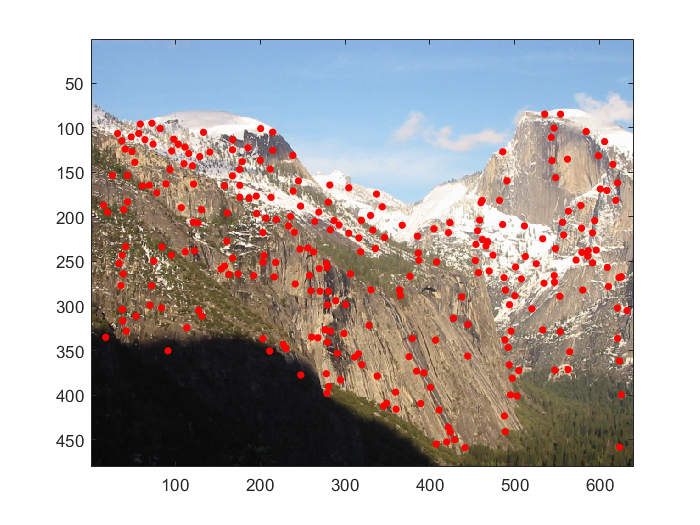
\includegraphics[width=.99\textwidth]{yosemite1_keypoints.png}
  \caption{Key points for given image yosemite1.}
\end{subfigure}%
\begin{subfigure}{.5\textwidth}
  \centering
  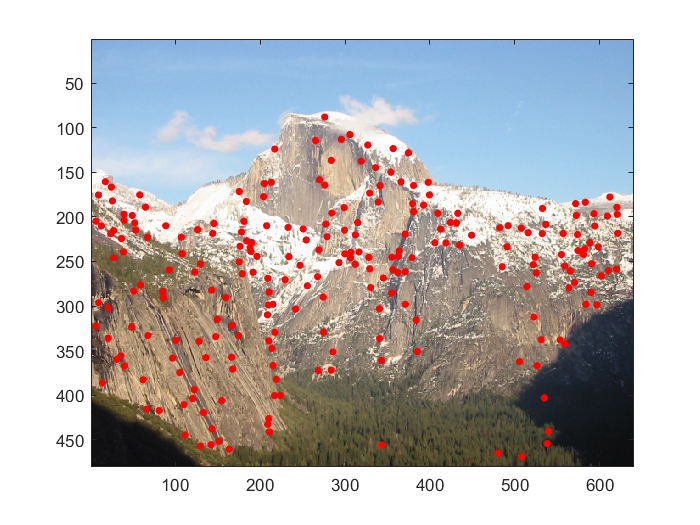
\includegraphics[width=.99\textwidth]{yosemite2_keypoints.png}
  \caption{Key points for given image yosemite2.}
\end{subfigure}
\caption{Visualization of key points extracted.}
\end{figure}

\newpage

\begin{figure}[!htb]
\begin{subfigure}{.5\textwidth}
  \centering
  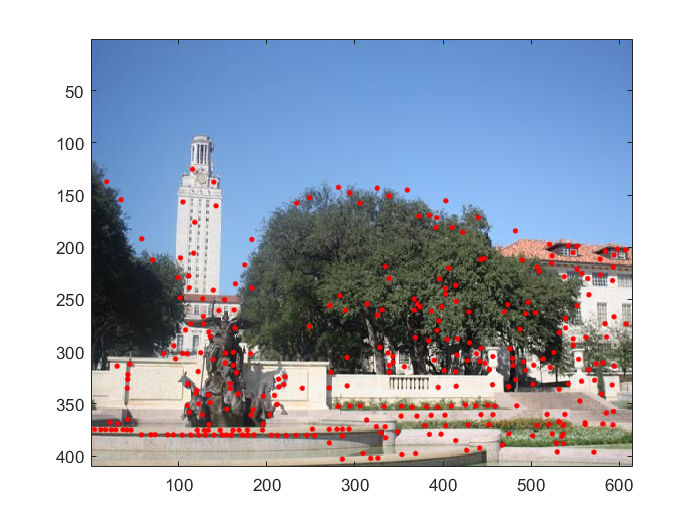
\includegraphics[width=.99\textwidth]{uttower2_keypoints.png}
  \caption{Key points for given original image of UT Tower.}
\end{subfigure}%
\begin{subfigure}{.5\textwidth}
  \centering
  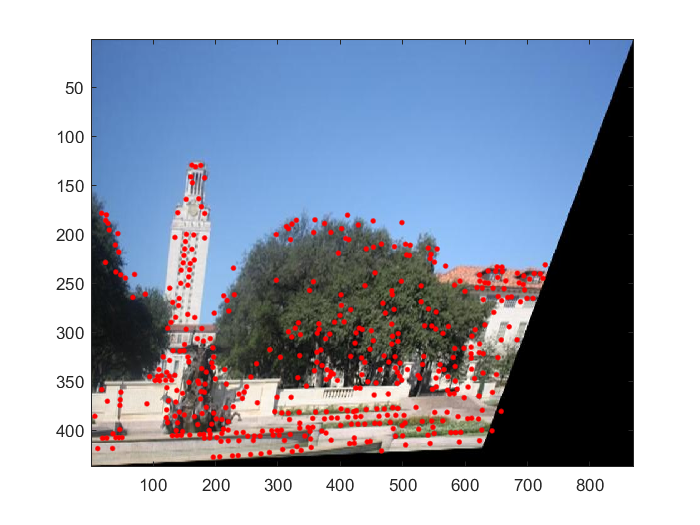
\includegraphics[width=.99\textwidth]{uttower2_bad_keypoints.png}
  \caption{Key points for disrupted image.}
\end{subfigure}
\begin{subfigure}{.9\textwidth}
  \centering
  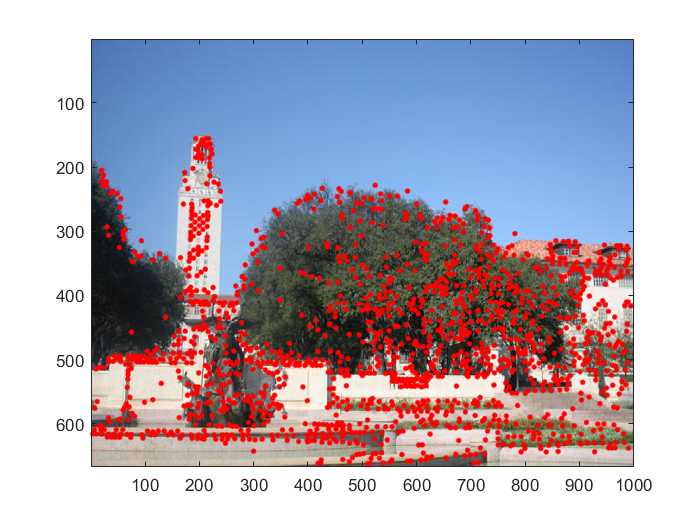
\includegraphics[width=.99\textwidth]{uttower2_scaledup_keypoints.png}
  \caption{Key points for scaled up image.}
\end{subfigure}
\caption{Visualization of key points extracted for different scales and orientations.}
\end{figure}

\newpage

\section{Feature Description}
\subsection{Algorithm}
For the second part we need to create SIFT descriptors from our key points. For this purpose, we will implement the algorithm from David G. Lowe's paper \href{``https://www.cs.ubc.ca/~lowe/papers/ijcv04.pdf}{Distinctive Image Features from Scale-Invariant Keypoints''}.
In summary, for each key point we detected from part one, we need to 
\begin{enumerate}
\item Take a NxN window around the key point, and normalize it to 16x16, where N is proportional to scale of key point.
\item Compute $ \nabla f(n_{1}, n_{2}) $ for each pixel in the window
\item Weight down the  $|\nabla f(n_{1}, n_{2})| $ of each pixel by a Gaussian function
\item For each pixel, compute edge orientation, i.e, $ \angle \nabla f(n_{1}, n_{2}) - \frac{\pi}{2}$ 
\item Create histogram of edge orientations within the window with 8 bins
\item Calculate the dominant direction using the histogram
\item Divide 16x16 window to four 4x4 cells
\item Compute a normalized orientation histogram for each cell (normalization is done by subtracting the dominant angle)
\end{enumerate}
to obtain a scale and orientation invariant descriptor. After these steps we will get a 128 dimensional (\#cells $\times $\#bins) descriptor for each key point. The implementation of this algorithm and helper functions used are given below.
\subsection{MATLAB Implementation}
\begin{lstlisting}[caption={General structure of the code for creating SIFT Descriptors.},captionpos=b]
function descriptors = SIFTDescriptor(pyramid, keyPt, keyPtScale)
% INPUT:
%   pyramid: Image pyramid. pyramid{i} is a rescaled version of the original image, in grayscale double format
%   keyPt: N * 2 matrix, each row is a key point pixel location in pyramid{round(scale)}. So pyramid{round(scale)}(y,x) is the center of the keypoint
%   scale: N * 1 matrix, each entry holds the index in the Gaussian pyramid for the keypoint. Earlier code interpolates things, so this is a double, but we'll just round it to an integer.
% OUTPUT:
%   descriptors: N * 128 matrix, each row is a feature descriptor

%% Initializations
% Number of keypoints that were found by the DoG blob detector
N = size(keyPt, 1);
% For each keypoint we will extract a region of size patch_size x patch_size centered at the keypoint.
patch_size = 16;
% The patch extracted around each keypoint will be divided into a grid of grid_size x grid_size.
grid_size = 4;
% Each histogram covers an area "pixelsPerCell" wide and tall
pixelsPerCell= patch_size / grid_size;
% The number of orientation bins per cell
num_bins = 8;
% Initialize descriptors to zero
descriptors = zeros(N, grid_size*grid_size*num_bins);

grad_mag = cell(length(pyramid),1);
grad_theta = cell(length(pyramid),1);
% Determine the gradient angles and magnitude of all images in the pyramid.
[grad_mag,grad_theta] = ComputeGradient(pyramid);

% Iterate over all keypoints
for i = 1 : N
    scale = round(keyPtScale(i));
    magnitudes = grad_mag{scale};
    thetas = grad_theta{scale};
    % Extract a patch of magnitudes and directions (16x16) around the keypoint
    [patch_mag,patch_theta] = Extract_Patch(keyPt(i,:),patch_size,magnitudes,thetas);
    if( isempty(patch_mag))
        continue;
    end
    % Normalize the gradient directions relative to the dominant gradient direction
    patch_theta = Normalize_Orientation(patch_mag, patch_theta);
    % Weight the gradient magnitudes using a Gaussian function
    patch_mag = patch_mag .* fspecial('gaussian', patch_size, patch_size / 2);
    % ComputeSIFTDescriptors for the patch, explanation is in the function implementation
    feature = ComputeSIFTDescriptor(patch_mag,patch_theta,grid_size,pixelsPerCell,num_bins);
    % Add the feature vector we just computed to our matrix of SIFT descriptors.
    descriptors(i, :) = feature;
end
% Normalize the descriptors.
descriptors = NormalizeDescriptors(descriptors);
end
\end{lstlisting}



\begin{lstlisting}[caption={My implementation of ComputeGradient function.},captionpos=b]
function [grad_mag,grad_theta] = ComputeGradient(pyramid)
%   Input:
%   pyramid: all the pyramid images in a cell array
%   Output:
%   grad_mag, grad_mag:
%       Two cell arrays of the same shape where grad_mag{i} and grad_theta{i} give the magnitude and direction of the i-th pyramid image. Gradient_angles ranges from 0 to 2*pi.
grad_theta = cell(length(pyramid),1);
grad_mag = cell(length(pyramid),1);
%Do this for all pyramid images
for scale = 1:length(pyramid)    
    currentImage = pyramid{scale};
    grad_mag{scale} = zeros(size(currentImage));
    grad_theta{scale} = zeros(size(currentImage));    
    % Discrete approximation of gradients
    img_dx = filter2([-1 0 1], currentImage);
    img_dy = filter2([-1; 0; 1], currentImage);
            
    grad_mag{scale} = sqrt(img_dx.*img_dx + img_dy.*img_dy);
    grad_theta{scale} = atan2(img_dy, img_dx) - deg2rad(90);        
    % atan2 gives angles from -pi to pi. To make the histogram code easier, we'll change that to 0 to 2*pi.
    grad_theta{scale} = mod(grad_theta{scale}, 2*pi);
end
end
\end{lstlisting}

\begin{lstlisting}[caption={My implementation for ComputeSIFTDescriptor function.},captionpos=b]
function descriptor = ComputeSIFTDescriptor(patch_mag,patch_theta,grid_size,pixelsPerCell,num_bins)
% INPUT:
%   patch_mag, patch_theta:
%       Two arrays of the same shape where patch_mag(i) and patch_theta(i) give the magnitude and direction of the gradient for the ith point. gradient_angles ranges from 0 to 2*pi
% OUTPUT:
%   descriptor: A 128 length descriptor calculated from 8-bin histograms of the 16 cells in the grid

% initialize descriptor to size 0
descriptor = [];
% iterate over each pixels
for x = 1 : grid_size
    % divide grid to cells
    cell_x_start = 1 + (x-1)*pixelsPerCell;
    cell_x_end = x * pixelsPerCell;
    for y = 1:grid_size
        cell_y_start = 1 + (y-1)*pixelsPerCell;
        cell_y_end = y * pixelsPerCell;
        % get cells from the grid
        mag_cell = patch_mag(cell_x_start:cell_x_end,...
            cell_y_start:cell_y_end);
        theta_cell = patch_theta(cell_x_start:cell_x_end,...
            cell_y_start:cell_y_end);
        % get the orientation histogram by using ComputeGradientHistogram
        cell_gradient_histogram = ComputeGradientHistogram(num_bins, mag_cell, theta_cell);
        % add descriptor of the cell to list of descriptors
        descriptor = [descriptor, cell_gradient_histogram];
    end
end
end
\end{lstlisting}

\newpage

\begin{lstlisting}[caption={My implementation of ComputeGradientHistogram function.},captionpos=b]
function [histogram, angles] = ComputeGradientHistogram(num_bins, gradient_magnitudes, gradient_angles)
% INPUT
% num_bins: The number of bins to which points should be assigned.
% gradient_magnitudes, gradient angles:
%       Two arrays of the same shape where gradient_magnitudes(i) and gradient_angles(i) give the magnitude and direction of the gradient for the ith point. gradient_angles ranges from 0 to 2*pi
%
% OUTPUT
% histogram: A 1 x num_bins array containing the gradient histogram. Entry 1 is the sum of entries in gradient_magnitudes whose corresponding gradient_angles lie between 0 and angle_step. Similarly, entry 2 is for angles between angle_step and 2*angle_step. Angle_step is calculated as 2*pi/num_bins.
% angles: A 1 x num_bins array which holds the histogram bin lower bounds. histogram(i) contains the sum of the gradient magnitudes of all points whose gradient directions fall in the range [angles(i), angles(i + 1))

angle_step = 2 * pi / num_bins;
angles = 0 : angle_step : (2*pi-angle_step);
histogram = zeros(1, num_bins);
% get sizes to use in loops
[size_x, size_y] = size(gradient_angles);
% iterate over all angles
for gradient_index_x = 1:size_x
    for gradient_index_y = 1:size_y
        grad_angle = gradient_angles(gradient_index_x, gradient_index_y);
        % start checking from biggest bin
        for angle_index = length(angles):-1:1
            if(grad_angle >= angles(angle_index))
                % update the bin value
                histogram(angle_index) = histogram(angle_index)...
                    + gradient_magnitudes(gradient_index_x, gradient_index_y);
                % we are done if our angle is bigger than or equal to bin lower bound
                break
            end
        end
    end
end
end
\end{lstlisting}

\newpage

\subsection{Sample Outputs}
\begin{figure}[!htb]
\begin{subfigure}{.5\textwidth}
  \centering
  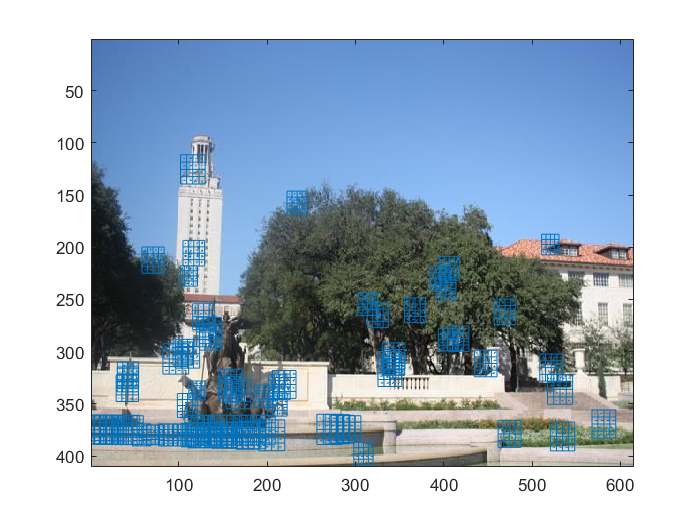
\includegraphics[width=.99\textwidth]{uttower2_sift.png}
  \caption{SIFT descriptors for given original image of UT Tower.}
\end{subfigure}%
\begin{subfigure}{.5\textwidth}
  \centering
  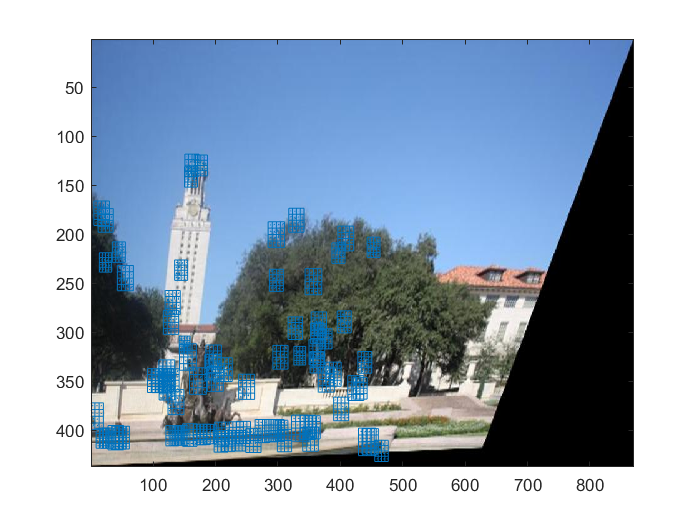
\includegraphics[width=.99\textwidth]{uttower2_bad_sift.png}
  \caption{SIFT descriptors for disrupted image.}
\end{subfigure}
\begin{subfigure}{.9\textwidth}
  \centering
  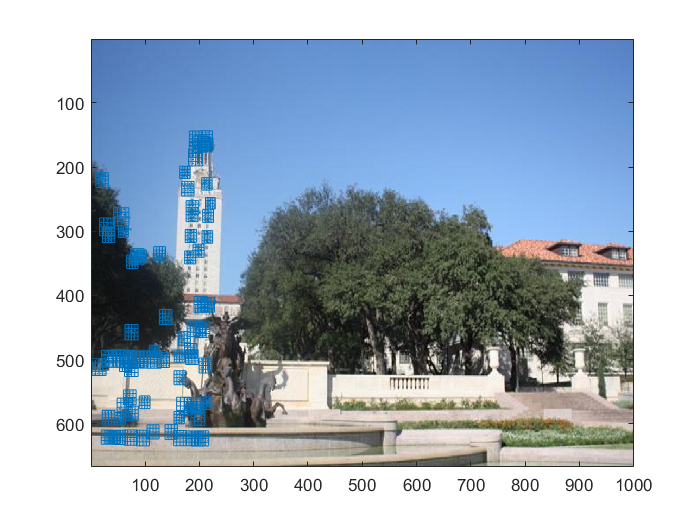
\includegraphics[width=.99\textwidth]{uttower2_scaledup_sift.png}
  \caption{SIFT descriptors for scaled up image.}
\end{subfigure}
\caption{Visualization of SIFT descriptors extracted for different scales and orientations.}
\end{figure}

\newpage


\begin{figure}[!htb]
\begin{subfigure}{.5\textwidth}
  \centering
  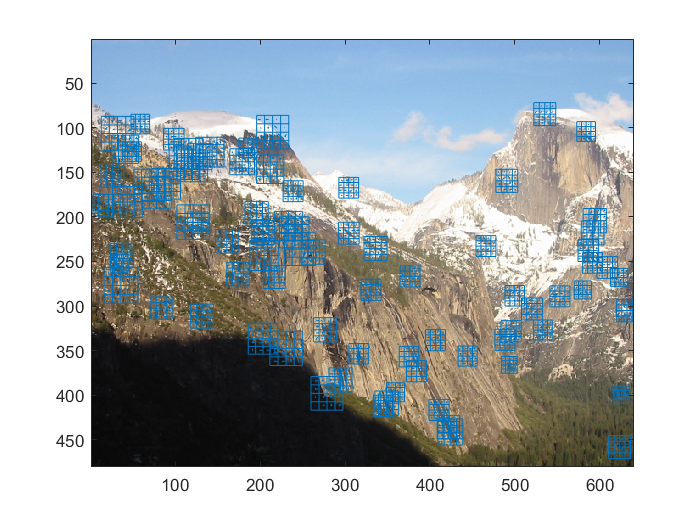
\includegraphics[width=.99\textwidth]{yosemite1_sift.png}
  \caption{SIFT Descriptors of given image yosemite1.}
\end{subfigure}%
\begin{subfigure}{.5\textwidth}
  \centering
  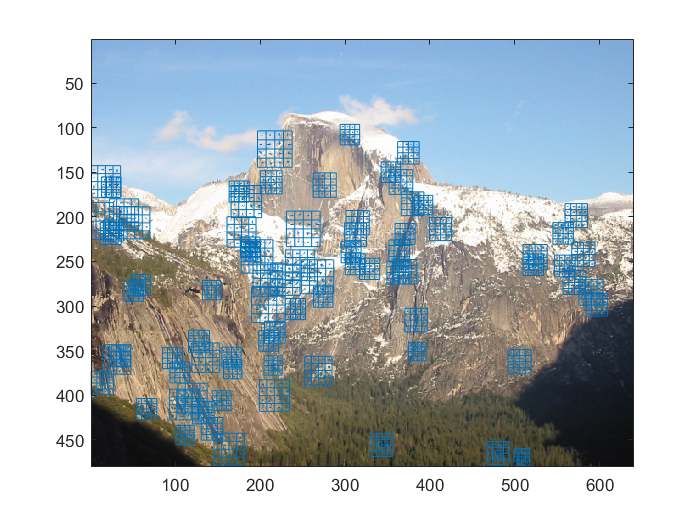
\includegraphics[width=.99\textwidth]{yosemite2_sift.png}
  \caption{SIFT Descriptors of given image yosemite2.}
\end{subfigure}
\begin{subfigure}{.5\textwidth}
  \centering
  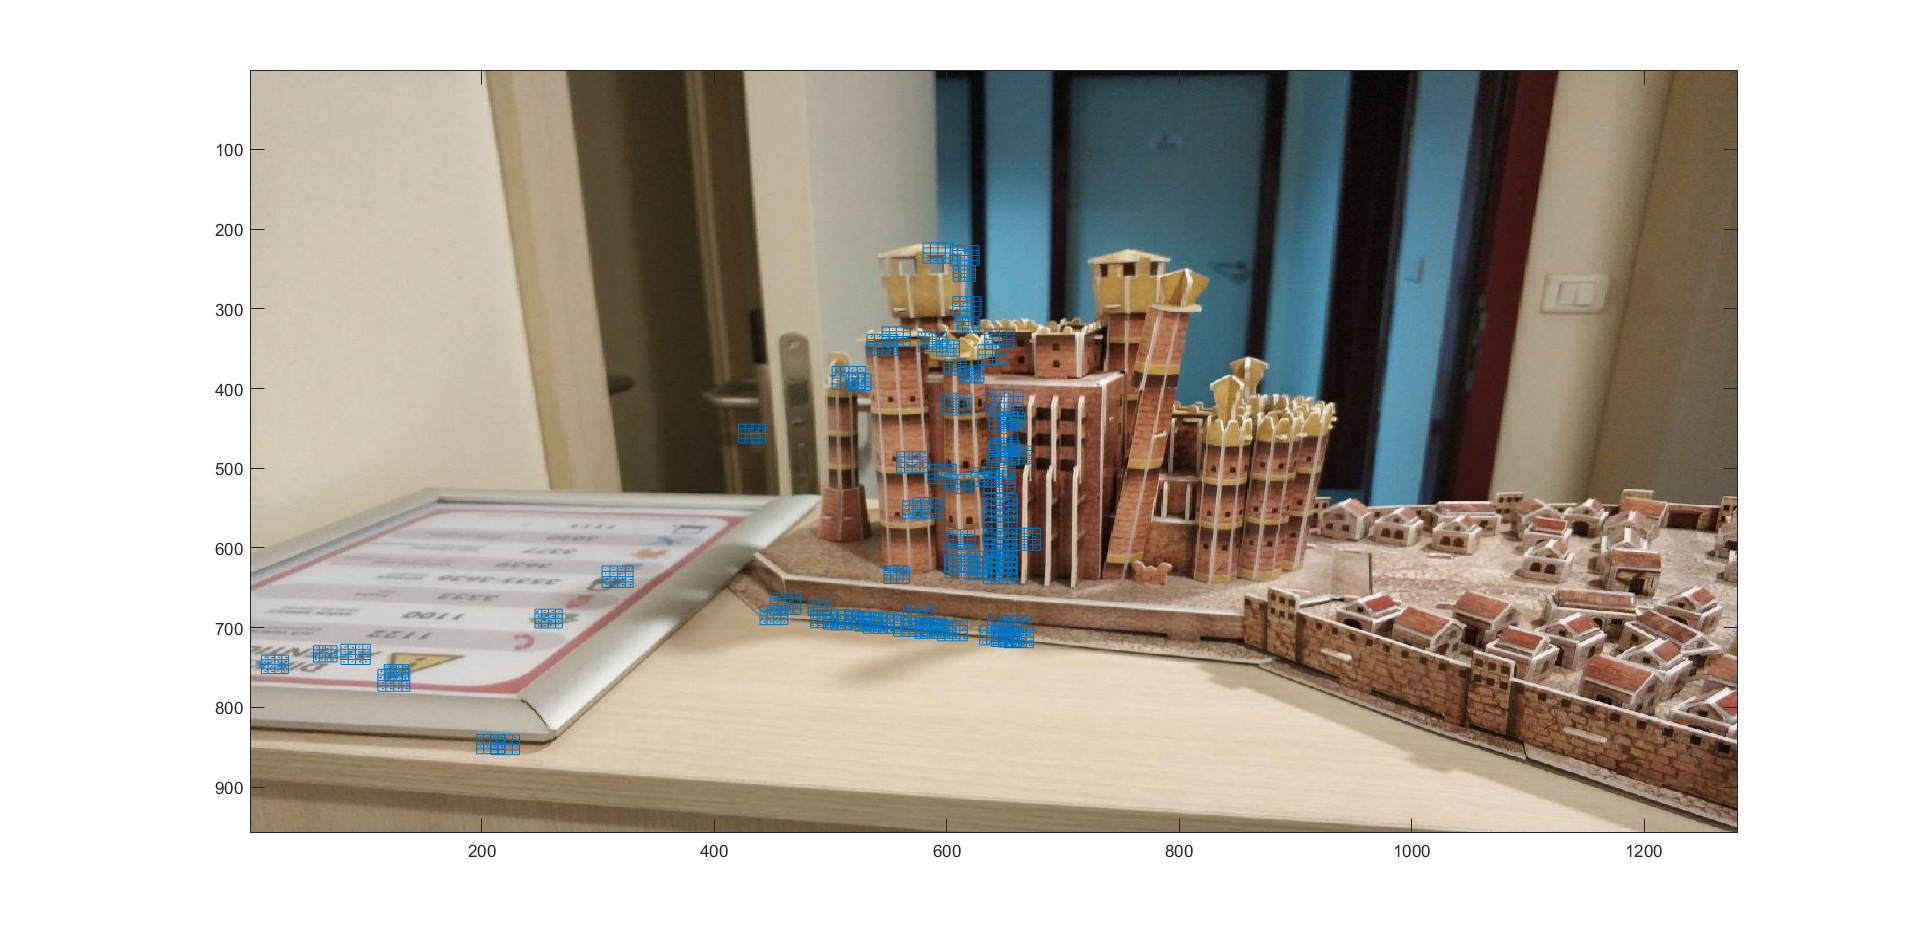
\includegraphics[width=.99\textwidth]{got1_sift.png}
  \caption{SIFT Descriptors of left part of King's Landing puzzle.}
\end{subfigure}%
\begin{subfigure}{.5\textwidth}
  \centering
  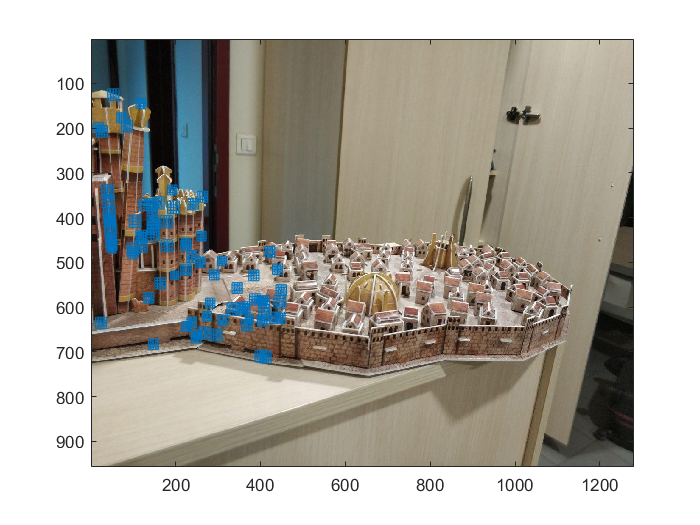
\includegraphics[width=.99\textwidth]{got2_sift.png}
  \caption{SIFT Descriptors of right part of the puzzle.}
\end{subfigure}
\caption{Visualization of SIFT Descriptors extracted.}
\end{figure}


\newpage

\section{Feature Matching}

\subsection{Algorithm}
The simple solution for feature matching is defining a distance function, such as Euclidean Distance, and iterate over all SIFT descriptors of second image to find the match for a descriptor in the first image. However, this simple solution is not the best, it can give good scores to bad matches. To decrease the number of false matches, we can use the ratio distance, i.e, the ratio of Euclidean distance between $f_{1}$ and $ f_{2}$ to Euclidean distance between $f_{1}$ and $f_{2}^{'} $, where $f_{1}$ is feature in first image,  $f_{2}$ is the best scored match to  $f_{1}$ according to distance function, and  $f_{2}^{'}$ is the second best match. We can filter false matches by eliminating the matches with ratios lower than some threshold value.

\subsection{MATLAB Implementation}

\begin{lstlisting}[caption={My implementation of SIFTSimpleMatcher function.},captionpos=b]
function match = SIFTSimpleMatcher(descriptor1, descriptor2, thresh)
% INPUT:
%   descriptor1: N1 * 128 matrix, each row is a SIFT descriptor.
%   descriptor2: N2 * 128 matrix, each row is a SIFT descriptor.
%   thresh: a given threshold of ratio. Typically 0.7
% OUTPUT:
%   Match: N * 2 matrix, each row is a match. For example, Match(k, :) = [i, j] means i-th descriptor in descriptor1 is matched to j-th descriptor in descriptor2.
    if ~exist('thresh', 'var'),
        thresh = 0.7;
    end
    match = [];
    %Get the number of descriptors for iterating
    [ld1, ~] = size(descriptor1);
    [ld2, ~] = size(descriptor2);
    for i = 1:ld1
        sift_desc_1 = descriptor1(i, :);
        %initilialize distances with infinity
        smallest = inf;
        second_smallest = inf;
        %initialize smallest index with zero
        smallest_index = 0;
        % this implementation assumes there are at least two descriptors in second array, smallest variables are wrong until end of first two iterations
        for j = 1: ld2
            sift_desc_2 = descriptor2(j, :);
            distances = sift_desc_1 - sift_desc_2;
            % dot product of row vector of distances with its transpose is equivalent with sum of squares of distances
            euclidian_dist = sqrt(distances * distances');
            % update values if necessary
            if (euclidian_dist < second_smallest)
                second_smallest = euclidian_dist;
            end
            if (euclidian_dist < smallest)
                second_smallest = smallest;
                smallest = euclidian_dist;
                smallest_index = j;
            end
        end
        % check ratio for threshold
        if (smallest < second_smallest * thresh)
            % add indexes of pair to match array if they pass the condition
            match = [match; [i, smallest_index]];
        end
    end
end

\end{lstlisting}
\subsection{Sample Outputs}

\begin{figure}[!htb]
  \centering
  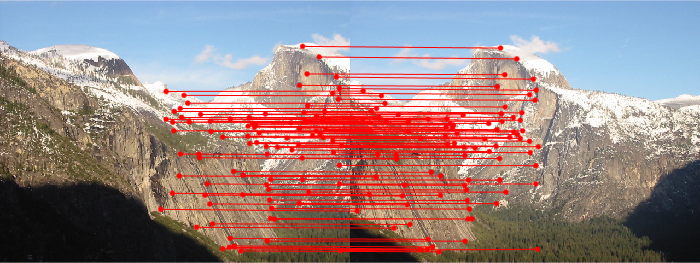
\includegraphics[width=.99\textwidth]{yosemite1_2_match.png}
  \caption{Visualization of matched key points between parts of Mount Yosemite.}
\end{figure}%
\begin{figure}[!htb]
  \centering
  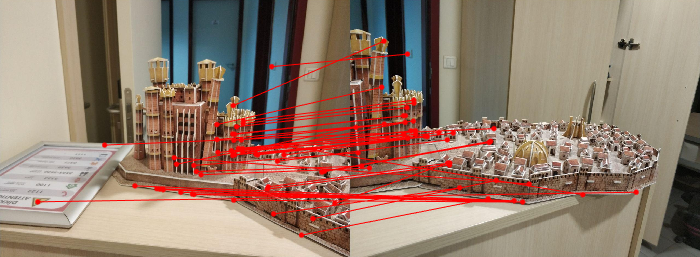
\includegraphics[width=.99\textwidth]{got1_2_match.png}
  \caption{Visualization of matched key points between parts of King's Landing Puzzle.}
\end{figure}%
\newpage
\begin{figure}[!htb]
  \centering
  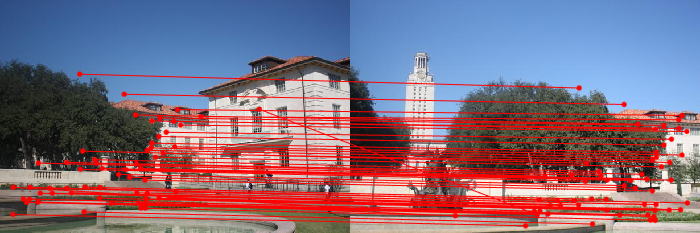
\includegraphics[width=.99\textwidth]{uttower1_2_match.png}
  \caption{Visualization of matched key points between parts of UT Tower.}
\end{figure}%
\begin{figure}[!htb]
  \centering
  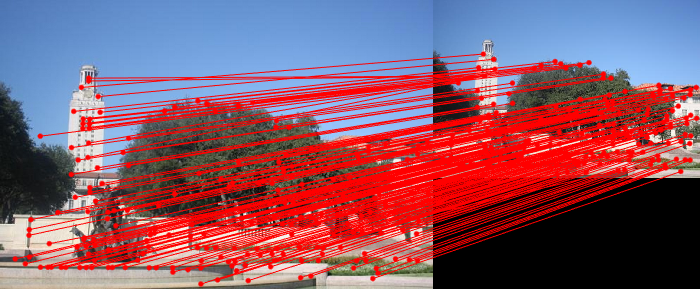
\includegraphics[width=.99\textwidth]{uttower2_2scaled_match.png}
  \caption{Visualization of matched key points between original and scaled UT Tower images.}
\end{figure}%
\begin{figure}[!htb]
  \centering
  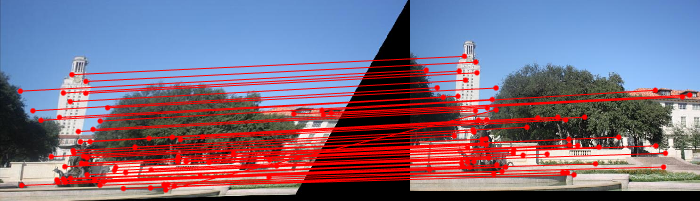
\includegraphics[width=.99\textwidth]{uttower2_2bad_match.png}
  \caption{Visualization of matched key points between original and disrupted UT Tower images.}
\end{figure}

As seen in the samples, SIFT Features are scale and rotation invariant.

\newpage

\section{Homography Estimation}

\subsection{Algorithm}
Homography is a mapping between two projection planes with the same center of projection, it can be represented as 3x3 matrix in homogeneous coordinates. A pixel in projection plane can be mapped to another projection plane with formula

$$
\begin{bmatrix} 
 wx^{'}  \\
 wy^{'}  \\
 w
\end{bmatrix}
=
\begin{bmatrix} 
  h_{00} & h_{01} & h_{02}  \\
   h_{10} & h_{11} & h_{12}  \\
    h_{20} & h_{21} & h_{22} 
\end{bmatrix}
\begin{bmatrix} 
 x \\
 y \\
 1
\end{bmatrix}
$$

So, we can estimate H by solving equations of the form: $wp_{i} = Hp_{i}$ using the matching pairs that we detected from previous parts. We will use RANSAC (Random Sample Consensus) algorithm to calculate H probabilistically. In RANSAC, we choose random n samples that it required to estimate H, and we will classify all the matches as inliers and outliers by thresholding them according to their errors. If the number of inliers exceed the threshold value, we will recalculate H using only the inliers. We repeat this procedure k times and keep the transformation with the minimum error.


\subsection{MATLAB Implementation}
\begin{lstlisting}[caption={My implementation of RANSACFit function.},captionpos=b]
function H_best = RANSACFit(p1, p2, match, seedSampleSize, maxInlierError, goodFitThresh )
% Input:
%   p1: N1 * 2 matrix, each row is a point
%   p2: N2 * 2 matrix, each row is a point
%   match: M * 2 matrix, each row represents a match [index of p1, index of p2]
%   seedSampleSize: The number of randomly-chosen seed points that we'll use to fit
%   maxInlierError: A match not in the seed set is considered an inlier if
%                   its error is less than maxInlierError. Error is
%                   measured as sum of Euclidean distance between transformed
%                   point1 and point2. You need to implement the
%                   ComputeCost function.
%   goodFitThresh: The threshold for deciding whether or not a model is
%                  good; for a model to be good, at least goodFitThresh
%                  non-seed points must be declared inliers.
% Output:
%   H: a robust estimation of affine transformation from p1 to p2

%% Initializations
N = size(match, 1);
if N<3
    error('not enough matches to produce a transformation matrix')
end
if ~exist('seedSetSize', 'var'),
    seedSampleSize = ceil(0.2 * N);
end
if ~exist('maxInlierError', 'var'),
    maxInlierError = 30;
end
if ~exist('goodFitThresh', 'var'),
    goodFitThresh = floor(0.7 * N);
end

%probability that all samples fail
p_fail = 0.001;
%fraction of inliers
w = 0.7;
%seed sample size
n = seedSampleSize;
% Determine the number of iterations required to ensure a good fit
maxIter = ceil(log(p_fail)/log(1 - w^n));
% initialize H with identity and error with infinity
H_best = eye(3);
min_error = inf;
% iterate maxIter times
for i = 1 : maxIter
    % Randomly select a seed group
    idx = randperm(size(match, 1));
    seed_group = match(idx(1:seedSampleSize), :);
    % Select remaining as the non-seed group
    non_seed_group = match(idx(seedSampleSize+1:end), :);
    % Use seed_group to compute the transformation matrix.
    H = ComputeAffineMatrix( p1(seed_group(:, 1), :), p2(seed_group(:, 2), :) );
    % Use non_seed_group to compute error from eucledian distance
    err = ComputeError(H, p1(non_seed_group(:, 1), :), p2(non_seed_group(:, 2),:));
    % Select the points as inliers which have error less than maxInlierError
    inliers = [];
    for index = 1:length(non_seed_group)
       if (err(index) < maxInlierError)
           inliers = [inliers; non_seed_group(index, :)];
       end
    end
    % recalculate H using only inliers if number of inliers is bigger than threshold
    number_of_inliers = size(inliers,1) + size(seed_group,1);
    if( number_of_inliers > goodFitThresh )
        all_inliers = [seed_group ; inliers];
        H = ComputeAffineMatrix( p1(all_inliers(:, 1), :), p2(all_inliers(:, 2), :) );
        err = ComputeError(H, p1(all_inliers(:, 1), :), p2(all_inliers(:, 2),:));
        % I used sum of squares of errors to evaluate H
        sum_err_squares = err' * err;
        if(sum_err_squares < min_error)
            min_error = sum_err_squares;
            H_best = H;
        end
    end
end
if sum(sum((H_best - eye(3)).^2)) == 0,
    disp('No RANSAC fit was found.')
end
end
\end{lstlisting}

\begin{lstlisting}[caption={My implementation of ComputeAffineMatrix function.},captionpos=b]
function H = ComputeAffineMatrix( Pt1, Pt2 )

N = size(Pt1,1);
if size(Pt1, 1) ~= size(Pt2, 1),
    error('Dimensions unmatched.');
elseif N<3
    error('At least 3 points are required.');
end
% Convert the input points to homogeneous coordintes.
P1 = [Pt1';ones(1,N)];
P2 = [Pt2';ones(1,N)];
% P1'*H' = P2' -> H' = P1'\P2'
H_transpose = P1'\P2';
H = H_transpose';
% Sometimes numerical issues cause least-squares to produce a bottom
% row which is not exactly [0 0 1], which confuses some of the later
% code. So we'll ensure the bottom row is exactly [0 0 1].
H(3,:) = [0 0 1];
end
\end{lstlisting}

\begin{lstlisting}[caption={My implementation of ComputeError function.},captionpos=b]
function dists = ComputeError(H, pt1, pt2)
% Input:
%   H: 3 x 3 transformation matrix where H * [x; y; 1] transforms the point
%   (x, y) from the coordinate system of pt1 to the coordinate system of pt2.
%   pt1: N1 x 2 matrix where each ROW is a data point [x_i, y_i]
%   pt2: N2 x 2 matrix where each ROW is a data point [x_i, y_i]
%   match: M x 2 matrix, each row represents a match [index of pt1, index of pt2]
% Output:
%    dists: An M x 1 vector where dists(i) is the error of fitting the i-th
%           match to the given transformation matrix.
%           Error is measured as the Euclidean distance
dists = zeros(size(pt1,1),1);
% Convert the input points to homogeneous coordintes.
pt1_homogeneous = [pt1' ; ones(1, length(pt1))];
pt2_homogeneous = [pt2' ; ones(1, length(pt2))];
% transform p1 using H
pt1_transformed = (H * pt1_homogeneous);

distances = pt1_transformed - pt2_homogeneous;
distances_x = distances(1, :);
distances_y = distances(2, :);
% distance_z is always all zero
% Calculate the Euclidean distances
% transpose the vector to satify documentation (return M x 1 matrix). 
dists = sqrt(distances_x .* distances_x + distances_y .* distances_y)';
if size(dists,1) ~= size(pt1,1) || size(dists,2) ~= 1
    error('wrong format');
end
end
\end{lstlisting}
\newpage

\section{Image Stitching}
We implemented all the necessary algorithms. We can stitch images by creating SIFT descriptors, performing feature matching, determining the transformation matrix H and finally using H to transform first image on top of second image. Code for this part is already given.

\subsection{Sample Outputs}
\begin{figure}[!htb]
  \centering
  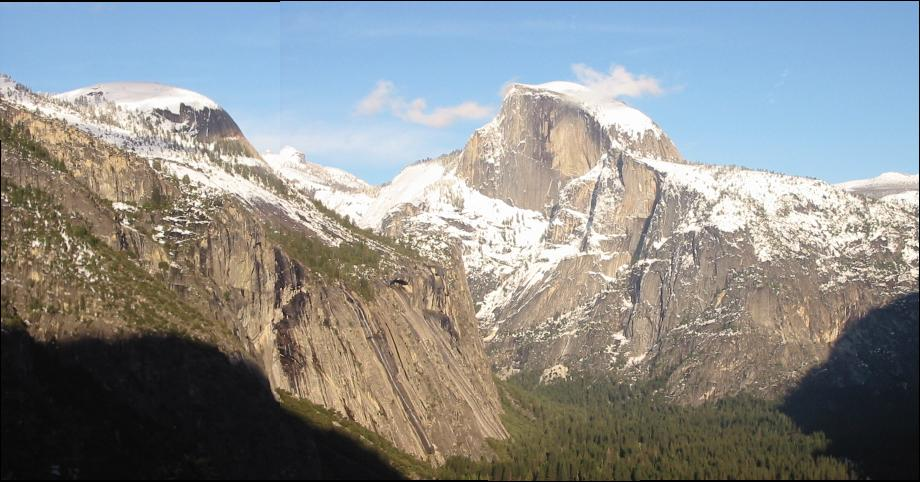
\includegraphics[width=.99\textwidth]{yosemite1_2_stitched.jpg}
  \caption{Stitched image of Mount Yosemite.}
\end{figure}%
\begin{figure}[!htb]
  \centering
  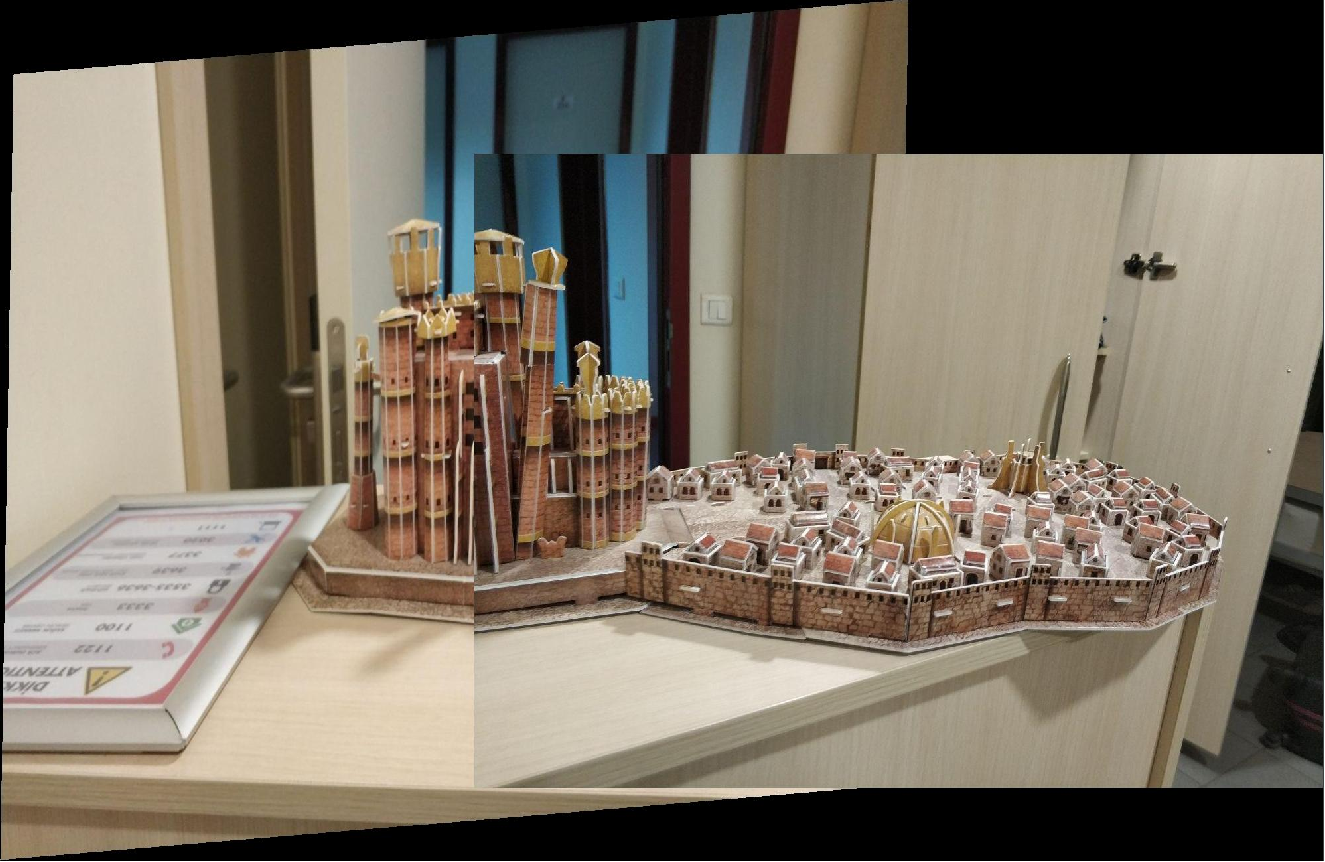
\includegraphics[width=.99\textwidth]{got1_2_stitched.png}
  \caption{Stitched image of King's Landing Puzzle.}
\end{figure}%
\newpage
\begin{figure}[!htb]
  \centering
  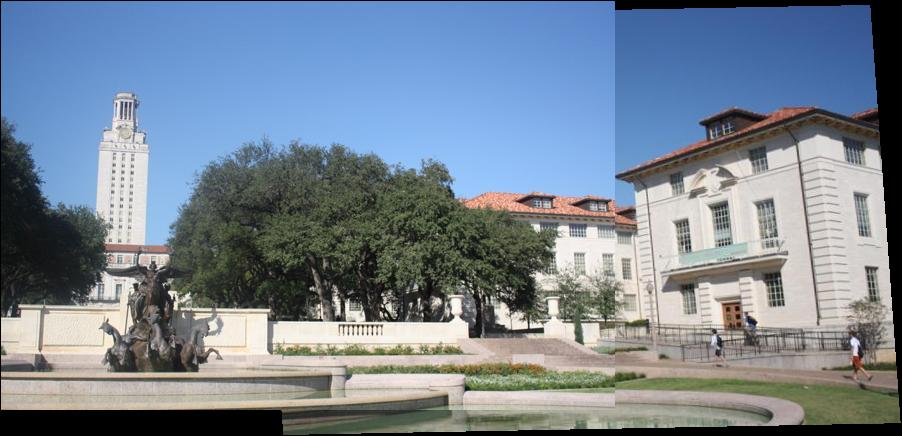
\includegraphics[width=.99\textwidth]{uttower1_2_stitched.jpg}
  \caption{Stitched image of UT Tower.}
\end{figure}%
\newpage

\section{Stitching Multiple Images}

\subsection{Algorithm}
We can simply stitch more than two images by first stitching two consequent images and continue until we are done. We can calculate homography matrices one for transformation in consequent images and use these matrices to transform all of the images to the same project plane.
\subsection{MATLAB Implementation}
\begin{lstlisting}[caption={My implementation of makeTransformToReferenceFrame function.},captionpos=b]
function T = makeTransformToReferenceFrame(i_To_iPlusOne_Transform, currentFrameIndex, refFrameIndex)
%makeTransformToReferenceFrame
% INPUT:
%   i_To_iPlusOne_Transform: this is a cell array where
%   i_To_iPlusOne_Transform{i} contains the 3x3 homogeneous transformation
%   matrix that transforms a point in frame i to the corresponding point in frame i+1
%   currentFrameIndex: index of the current coordinate frame in i_To_iPlusOne_Transform
%   refFrameIndex: index of the reference coordinate frame
% OUTPUT:
%   T: A 3x3 homogeneous transformation matrix that would convert a point
%   in the current frame into the corresponding point in the reference
%   frame. For example, if the current frame is 2 and the reference frame
%   is 3, then T = i_To_iPlusOne_Transform{2}. If the current frame and
%   reference frame are not adjacent, T will need to be calculated.

T = eye(3);
% if target index is bigger than current index, iteratively multiply transformation matrix with T from left until new matrix until goal is reached 
if (currentFrameIndex < refFrameIndex)
   for i = currentFrameIndex:refFrameIndex - 1
      T =  i_To_iPlusOne_Transform{i} * T;
   end
 % if target index is lower than current index, first find the inverse of transformation matrix and multiply it with T from left until goal is reached
elseif (currentFrameIndex > refFrameIndex)
    for i = currentFrameIndex - 1: -1:refFrameIndex
      T =  pinv(i_To_iPlusOne_Transform{i}) * T;
    end
end
end
\end{lstlisting}

\newpage

\subsection{Sample Outputs}
\begin{figure}[!htb]
  \centering
  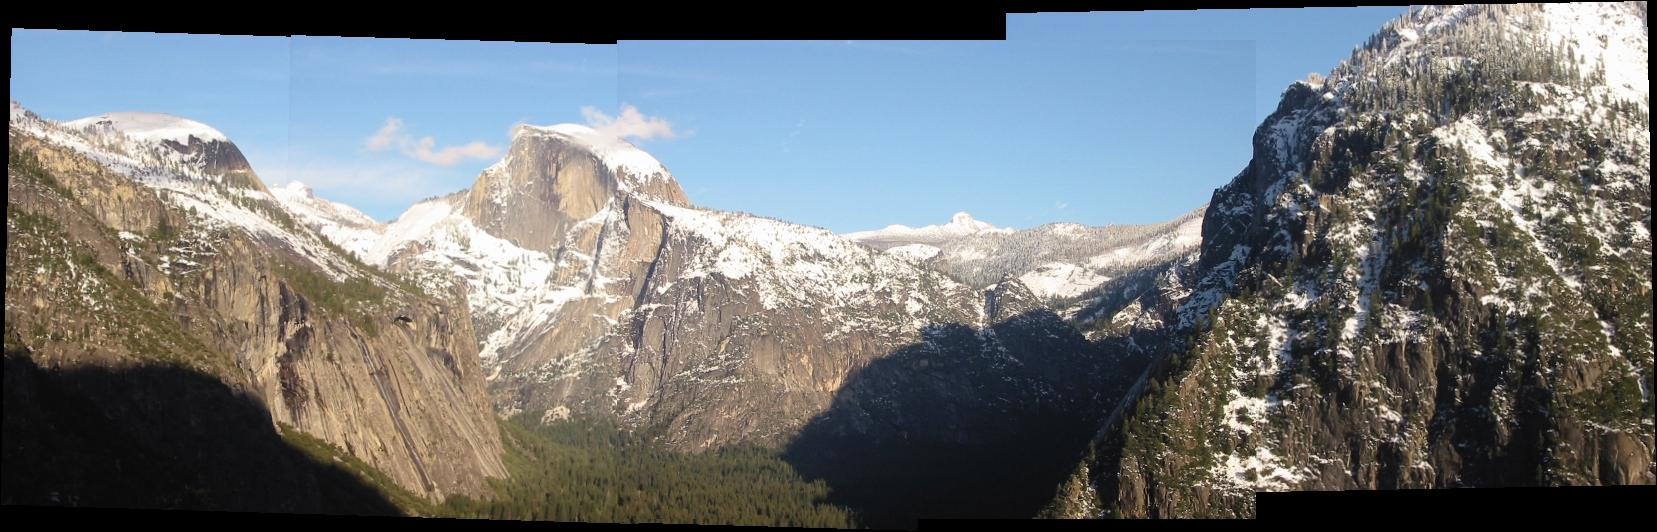
\includegraphics[width=.99\textwidth]{yosemite_pano.jpg}
  \caption{Stitched image of Mount Yosemite from multiple images.}
\end{figure}%
\begin{figure}[!htb]
  \centering
  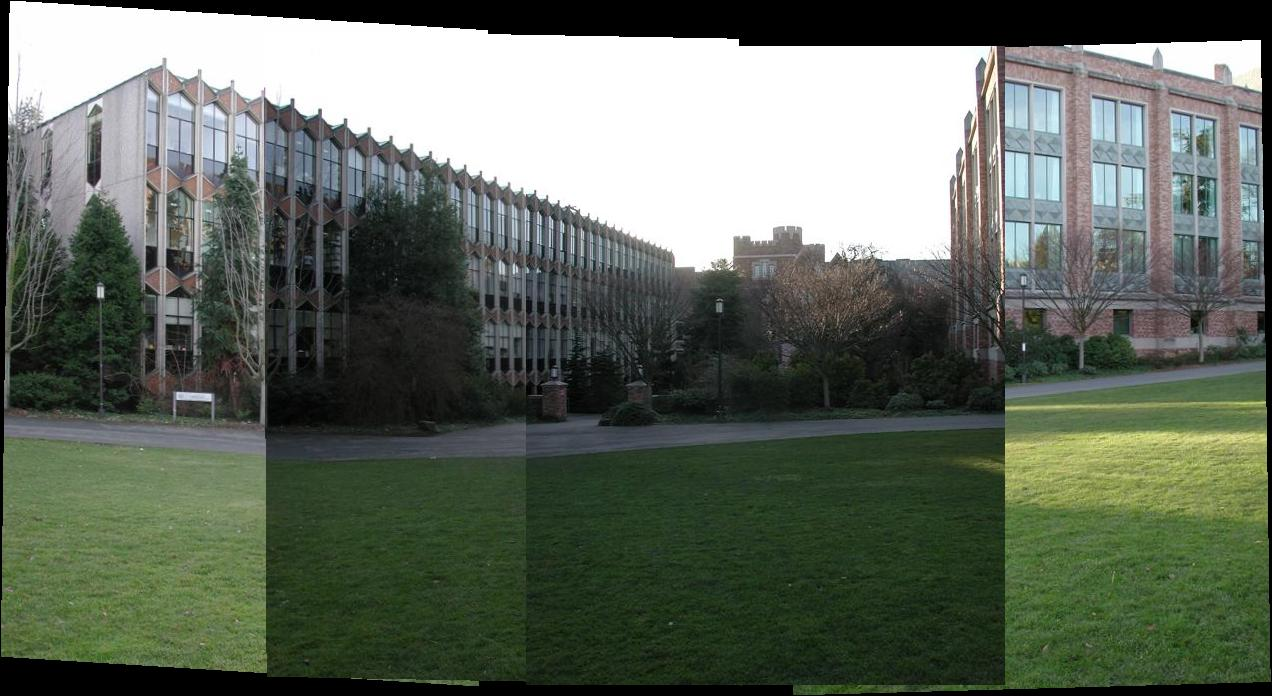
\includegraphics[width=.99\textwidth]{campus_pano.jpg}
  \caption{Stitched image of campus from multiple images..}
\end{figure}%
\newpage
\begin{figure}[!htb]
  \centering
  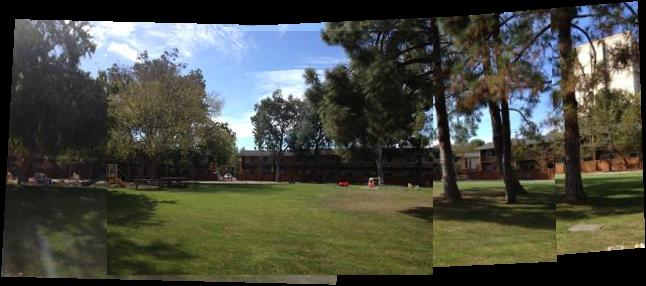
\includegraphics[width=.99\textwidth]{yard_pano.jpg}
  \caption{Stitched image of yard from multiple images.}
\end{figure}%
\section{Principal Component Analysis}





\end{document}